\documentclass[11pt]{article}
\usepackage[scale=0.75,twoside,bindingoffset=5mm,a4paper]{geometry}
\usepackage[utf8]{inputenc}
\usepackage{kotex}
\usepackage{lmodern}
\usepackage{cite}
\usepackage{minted}
\usepackage{graphicx}

\author{20193601 지준섭}
\title{HeyMoney: Automatic Debt Management System With Messenger Conversation \\
\begin{large}
  CS579 Homework\#5: Final Report
\end{large}}

\begin{document}

\maketitle

\begin{abstract}
  It is necessary to treat a financial relationship problem as a person
  belong to the groups, circles, or the companies.
  In this project, we build a ssystem that manages the debt and the credit automatically.
  The system parses the natural language in the messenger \textit{Slack}
  using definite clause grammar(DCG), and generates an appropriate transaction.
  The system also provides a web page to view the user's current status.
  Users do not need to learn how to use the system, such as memorizing commands,
  they can just use familiar natural language to manage the money.
\end{abstract}


\section{Introduction}

While a person belongs to groups, such as circles or the companies,
there is always a problem of financial relationship.
The problem can be about a dinner eaten together,
a product purchased on behalf of another, etc.
When these money records are made, a person need to memorize or take notes of them.
Only two or three records may not be a problem,
it is hard to manage many records of debts and credits however.

So it must be useful when we build a system of managing financial records,
that automatically generates financial records and provides the summary page.
On the other hand, there must be a problem for developing the new system --
the users must learn how to use the system.
For example, most chat-based system needs to type commands with custom defined
rules. Also web or application based system needs to learn
which button is needed to be clicked.

To solve this problem, we decided to implement a natural language based system.
The user does not need to learn the extra requirements to use the service.
We implement some prolog based rules to parse the messages,
and a database-related system which generates or kills the
transactions(money records) not manually.

\section{Requirements}

Briefly, our system has four big requirements to achieve:

\begin{enumerate}
  \item \textbf{The system should see whether the message is about money or not.}
  In the messenger, there are also messages not related with financial problems.
  The system should distinguish the text is about financial relation or not.
  \item \textbf{The system should extract the amount of money from the message.}
  We assume that there is always a number in the money-related conversation
  which describes the amount of the debt or the credit.
  The parser must extract the amount of money for each text
  and apply it to the transaction.
  \item \textbf{The system should notice which word is the people's name,
  and which word is the item's name.}
  For each transaction, we assume that there always exists
  a creditor and a debtor, and a item if the text is making a new debt.
  For example, thinking about a sentence
  `Mia: @John, give me 5 dollars for dinner.',
  we can see that the person who speaks, \textit{Mia}, is a creditor.
  And it is trivial that \textit{John} is a debtor, and \textit{dinner}
  is the item's name.
  Our parser must find out such information and process generating, or deleting
  the transaction.
  \item \textbf{The system must cover three different fields:
  \textit{Slack} as a messenger, transactions database, and the webpage.}
\end{enumerate}

\section{Structure \& Scenario}

Figure \ref{fig:diagram} briefly represents the structure of our system -- \textit{HeyMoney}.

\begin{figure}[!htbp]
  \centering
  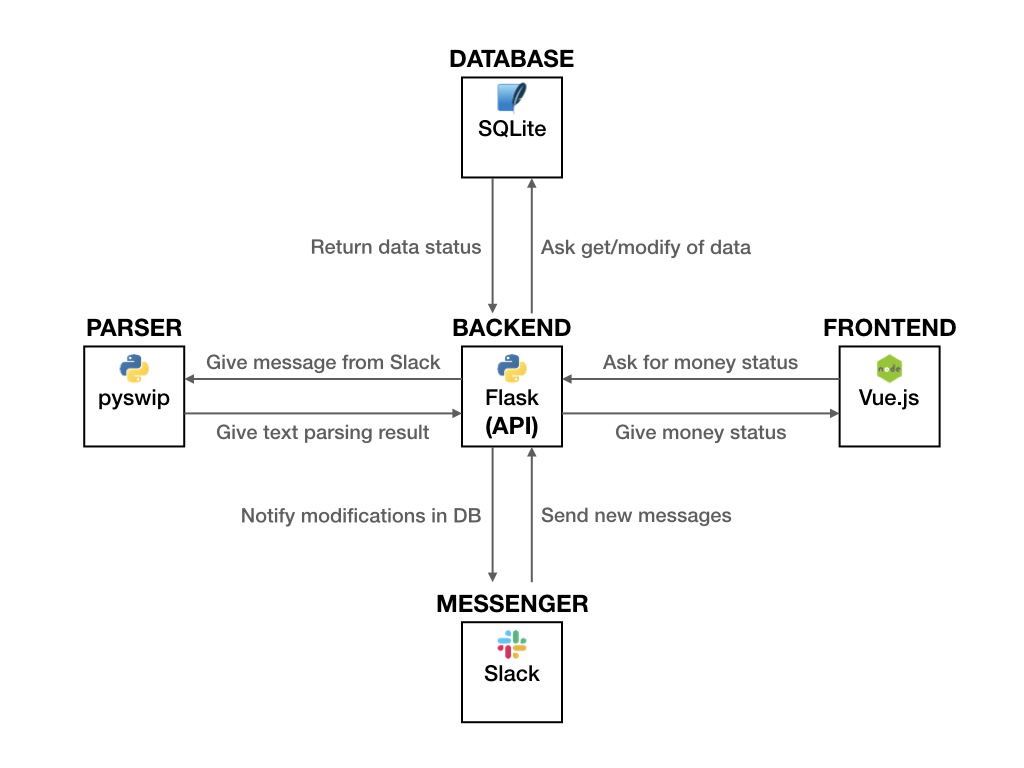
\includegraphics[width=\textwidth]{images/cl-hw3-diagram.png}
  \caption{The diagram of \textit{HeyMoney} system.}
  \label{fig:diagram}
\end{figure}

\subsection{Structure}

\subsubsection{Messenger -- \textit{Slack}}

For the project, we have to select a particular messenger for the development.
The messenger should satisfy these conditions:
\textbf{1.} should be widespread --
the system will become more useful when the more people use the messenger.
\textbf{2.} must provide an API and documents;
This feature makes us easy to debug and add functionalities.
So we choosed a \textit{Slack} to play a role of messenger.
\textit{Slack} is a widely-known for groups,
such as circles, laboratories, and companies.
It provides an official API and documentation
for accessing the messages in the channel,
so people can easily build a bot when they need a special function.

\subsubsection{Parser -- \textit{SWI-prolog}}
Our system will receive the \textit{Slack} messages as input.
The message will have some attributes -- a \textit{username}, a \textit{timestamp},
and a \textit{body text}.
The \textit{username} is an unique id for the user,
the \textit{timestamp} represents a time the message sended,
and the \textit{body text} is in natural language form,
and parsing this feature will be our main challenge of the project.

The parser will extract the information such as
\textit{who(debtor) should give creditor a money}, and \textit{the amount of money}.
To do this, we will use a concept of Definite Clause Grammar(DCG), and customize it.
For example, let's think about some sentences,
\textit{``@John, please give 3 dollars for lunch.''},
and \textit{``I gave @Mike 3 dollars''}.
With DCG, we can extract some noun phrases like
\textit{@John}, \textit{lunch}, \textit{I}, and \textit{@Mike}.
They are noun phrases, and \textit{I} is especially pronouns.
In these sentences, we can assume that the pronouns mean the sender of the message.
Also, we can extract the amount of money like \textit{3 dollars}.
Then the sentences can be represented like \textit{`debt(@john, Sender, 3, lunch)'},
and \textit{`pay(Sender, @mike, 3)'}. And these representations will
make the database add a debt/pay log.

We decided to use \textit{SWI-prolog} language for our parser,
because the language is optimized to parse and extract the information
from such sentences.

\subsubsection{Backend -- \textit{Flask}}
The backend server plays most of the role in this system.
It should communicate with four other parts of the system:
the messenger, the parser, the database, and the frontend server.
With the messenger, it receives new messages from messenger,
and send results of the DB modification(notifications) to the messenger.
With the parser, it sends the data(message) to the parser,
and receives the parsed result.
If the parsed result is valid, the backend should interact with database.
It sends the request of modifying the data to the database,
and get a result of request.
Sometimes the frontend server makes an API call to get the status of the debt,
such as a summarization, or statistics.
Then the backend will make some requests of getting data, process it, and send the result back.
To achieve these features, we selected Flask as a Python library,
because it enables an effective develpment and a big extensibility.

\subsubsection{Database -- \textit{SQLite}}
The database saves all the logs of debt and payment.
When the request originally from the frontend server arrives, the database
will calculate the stats based on the query and return the result.
When the request is from the parser, the database will add a row to the
debt or the pay collection.
The new row should include the debtor and creditor, amount of debt,
and the time when the message was sent.
We choose \textit{SQLite} as the database of the system,
because it allows us easier data management with just one file.

\subsubsection{Frontend -- \textit{Vue.js}}
User must want to see their debt status in a readable form.
The frontend server is a solution for this demand.
The server send database a request to get the statistics through the backend,
and represent the result in a readable form: such as tables and graphs.
The components can be about total statistics of the group, or about a user.
\textit{Vue.js}, a library of \textit{Node.js} will just fit for this performance.
The library requires less communication with the backend server,
so it is easy to optimize the speed of the application.
Also, there is a lot of graph modules can be attached to the \textit{Vue.js}.


\subsection{Scenario}
\subsubsection{The user requests money to other people}
For example, a user buys a dinner to eat with two people together,
and want to ask for a money.
The user \textit{@Mia} can say ``@John, give me 20,000 won for dinner.''.
The system should analyze this kind of request,
and assign a proper amount of money to the debtor.
Both sentences will be represented as \textit{`debt(@john, @mia, 20000)'},
and the debt log will be added to the database.

\subsubsection{The user wants a notice that he/she has paid the debt}
After sending a proper money to the creditor,
the debtor \textit{@john} will say ``I just sent 10,000 won to @Mike.'', 
This sentence can be represented as \textit{`pay(@john, @mike, 10000)'}.
Before adding the payment log to the database, our system must check that
the sender really has the same or over 10,000 won debt to Mike.

\subsubsection{The user wants to view the debt summary}
In this case the user should access the web application.
The webpage should show the summary of debt/receivables,
and detailed information of each transaction, such as date, amount, item, and person.


\section{Implementation Details}

\subsection{Messenger}

We use a Python library to a \textit{Slack}, called \textit{python-slackclient}
to build a bot, receiving messages and replying.
I use a custom \textit{Slack} server that I have a permission,
and generate an API key for the bot.
When the message event has detected,
the bot call parser and watch the result.
If the message is identified as money-realted, the bot makes a new transaction,
or kills the existing transaction.
This process must have database as co-worker, so we use another Python library
called \textit{sqlalchemy} to communicate with database.
The reason why we chose \textit{sqlalchemy} is,
we can still modify the database with the same code
even if the engine of database has changed, for example, from SQLite to MySQL.
Also \textit{sqlalchemy} has its own logic to check the security,
so our system will become much safer than using the raw query to the database. 


\subsection{Parser}

At first we tried to use the Python library that ables Prolog program execution
in Python code, call \textit{pyswip}. But due to the minor support of the library,
the program continously made a \textit{core dumped} error.
After many tries, we decided to call raw \textit{SWI-prolog} program
witth a subprocess of the Python slackbot program.

Briefly, we build two kind of parser, the first one is for generating debt --
such as the sentence `@John, give me 5000 won for dinner.'. And here is the example.

\begin{minted}{prolog}
s(User, Price, What) --> user(User), givep(Give), pricep(Price), whatp(What).

user(User) --> [User].

givep(Give) --> give(Give), me(Me).
givep(Give) --> manner(Manner), givep(Give).
manner(Manner) --> [Word], {lex(Word, mannerword)}.
give(Give) --> [Word], {lex(Word, giveword)}.
me(Me) --> [Word], {lex(Word, meword)}.

pricep(Price) --> price(Price), won(Won).
price(Price) --> [Price].
won(Won) --> [Word], {lex(Word, wonword)}.

whatp(What) --> for(For), what(What).
for(For) --> [Word], {lex(Word, forword)}.
what(What) --> [What].

lex(please, mannerword).
lex(just, mannerword).
lex(should, mannerword).
lex(must, mannerword).
lex('Give', giveword).
lex(give, giveword).
lex(grant, giveword).
lex(donate, giveword).
lex(me, meword).
lex(won, wonword).
lex(for, forword).
\end{minted}

As we can see, we parse the sentence into four phrase:
user phrase, give phrase, price phrase, and what phrase.
At first the user phrase parses who is the debtor.
After that, parser finds out the `give' words, such as \textit{give},
\textit{grant}, or \textit{donate}.
According to the code above, the parser can parse some `manner words',
such as \textit{please}, \textit{just}, \textit{should}, or etc.
These `manner words' are not necessary, but human can use it to show
their politeness or significantness of the transaction.
Then the parser extracts the price of the transaction, and at last
finds out the name of the item, in the `what phrase'.

And here is the example parser for killing transaction:

\begin{minted}{prolog}
s(User, Price) --> i(I), sendp(Send), pricep(Price), userp(User).

i(I) --> [Word], {lex(Word, iword)}.

sendp(Send) --> send(Send).
sendp(Send) --> manner(Manner), sendp(Send).
manner(Manner) --> [Word], {lex(Word, mannerword)}.
send(Send) --> [Word], {lex(Word, sendword)}.

pricep(Price) --> price(Price), won(Won).
price(Price) --> [Price].
won(Won) --> [Word], {lex(Word, wonword)}.

userp(User) --> to(To), user(User).
to(To) --> [Word], {lex(Word, toword)}.
user(User) --> [User].

lex('I', iword).
lex(i, iword).
lex(just, mannerword).
lex(have, mannerword).
lex(sent, sendword).
lex(granted, sendword).
lex(donated, sendword).
lex(won, wonword).
lex(to, toword).
lex(for, toword).
\end{minted}

As we can see, the sentence is constructed with four phrases:
`I' phrase, send phrase, price phrase, and the user phrase.
When the parser find `I' in the beginning of the sentence,
parser continously finds `send words', and extract the amount of money
after those words.
Finally, the parser extracts the user as creditor from the sentence.

\subsection{Backend}
We use \textit{Flask}, and \textit{Flask-RESTful} from Python to build a backend server.
As same as the \textit{Slack} bot part, we use \textit{sqlalchemy} to communicate with database.
Our backend gets the data from the database, and provide it in JSON form to the frontend.

\begin{minted}{json}
[
  {
    "tid": 6,
    "name": "playstation",
    "creditor_id": "URKP3BAFJ",
    "debtor_id": "U6HB7CTRT",
    "price": 390000,
    "timestamp": 1576133730
  },
  {
    "XXX": "..."
  }
]
\end{minted}

Above is the example of calling transactions with creditor id = URKP3BAFJ.
There are price of the item, name of the item, creditor and debtor.

\subsection{Database}
The database is managed with the engine \textit{SQLite}.
We chose it because \textit{SQLite} only needs one file to make a database;
It allows simple and easy way to manage the database.
There are three tables in the database: \textbf{Users}, \textbf{Transactions},
and \textbf{Dead Transactions}.
The \textbf{Users} table saves user's basic information,
such as uid, name, total debt and credit.
The \textbf{Transactions} table saves the records information,
transaction id, name, price, timestamp, and ids of the creditor and debtor.
And the third one \textbf{Dead Transactions} saves dead, or the paid transactions.
When the transaction is paid, it is `killed'.
It is removed from the \textbf{Transactions} table and added to the 
\textbf{Dead Transactions} table.

\subsection{Frontend}
\textit{Vue.js}, a javascript(node.js) framework is playing a role of frontend.
It calls an API, provided by backend server when the page is called by a user.
When the frontend gets the raw JSON data, the engine of the browser
assign the values to the proper element in the web page.
The frontend shows four big component in the web page: total debts of the user,
total credits of the user, the list of debts, and the list of credits.

\section{Result}
With the process above, we build a full-stack, well made system for debt management.
When the creditor wants debtor to pay, just say like Figure \ref{fig:creditor}.

\begin{figure}[!htbp]
  \centering
  \includegraphics[width=0.6\textwidth]{images/creditor.jpg}
  \caption{Creditor wants a debtor to pay.}
  \label{fig:creditor}
\end{figure}

Then the new transaction -- has `playstation' as attribute, 400,000 won for
price -- will be added to database.

If the debtor wants to notice the creditor that the debtor paid,
he or she will type just like Figure \ref{fig:debtor}.

\begin{figure}[!htbp]
  \centering
  \includegraphics[width=0.6\textwidth]{images/debtor.jpg}
  \caption{Debtor wants a notice for payment.}
  \label{fig:debtor}
\end{figure}

With this message, our system will reduce the debts from the transaction.
After all process done, user can see the summary of his/hers status,
like Figure \ref{fig:summary}.

\begin{figure}[!htbp]
  \centering
  \includegraphics[width=\textwidth]{images/web.jpg}
  \caption{Summary view.}
  \label{fig:summary}
\end{figure}

\section{Conclusion}
With the implmented system, user can easily manage their
financial relationship using their familiar things -- messenger, web, and
the most important one, natural language.
It will be really useful for groups with not big number of members,
such as circles, laboratories, or the group of friends.
Now we think we can improve the system for more specific situations.
Sometimes people want to mention two or more people in one message,
and the amount of money in the message should be divided by the number of people
or stay still. To decide whether or not to divide the amount of money,
the understanding of sentence is needed.
Adding more complex rules for the parser may help the problem.
Also, supporting more language may be a interesting topic.
For implementation, we felt that executing SWI-prolog as subprocess of Python
is not effecient for the system. We found that there is javascript adopted
version of prolog, so maybe next time we will try it.

\end{document}